\section{Conception de la classe \textit{CPincePrehension}}
\label{sec:pince_prehension}

\begin{center}
    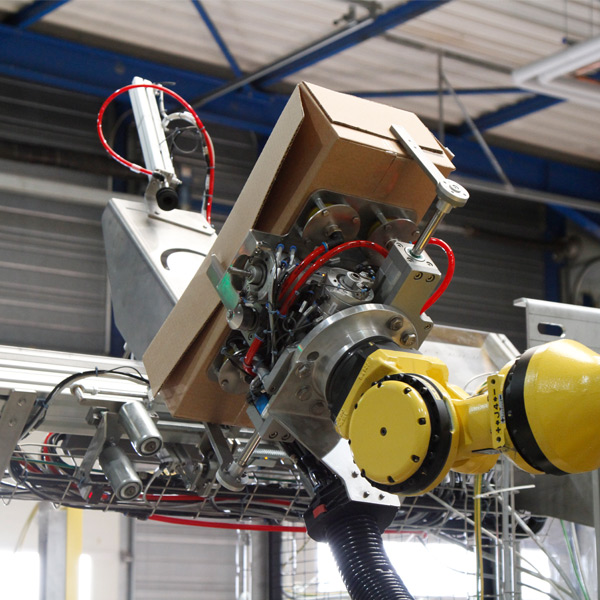
\includegraphics[width=0.7\textwidth]{figures/prehenseur.jpg}
\end{center}

On s'intéresse ici à la modélisation de la pince de préhension du robot. Cette pince est utilisée pour saisir et maintenir les cartons ouverts pendant le processus de vidage.
\subsection*{Description de la pince de préhension}
La pince de préhension est équipée d'un système de préhension par ventouses et de deux paires de bloqueurs.

Le \textbf{système de préhension} par ventouses permet de saisir le carton en appliquant une pression négative pour créer une adhérence. Il est piloté à l'aide d'un distributeur pneumatique qui contrôle l'aspiration et la libération des ventouses. Un capteur de pression est utilisé pour vérifier si le carton est correctement saisi.

Pour les bloqueurs de volets (au nombre de 4), on propose d'utiliser des vérins roto-linaires. Ce sont des vérins permettant une translation linéaire et une rotation. Ils sont utilisés pour maintenir les volets du carton ouverts pendant le processus de vidage. Chaque paire de bloqueurs est contrôlée par un vérin distinct, permettant ainsi de maintenir les volets en position ouverte.

